%!TeX root = ../principal.tex
%!TeX encoding = utf-8
\chapter{Classe FEECTeX}
\label{cap1}

\section{Citações}

Considerando que as referências estejam armazenadas no arquivo \textit{bibliografia.bib} na pasta raíz, as citações podem ser feitas através dos comandos:

\begin{itemize}
    \item \verb|\citar{<chave#1>, <chave#2>, ..., <chave#n>}|;
    \item \verb|\citarautora{<chave>}| ou \verb|\citarautor{<chave>}|;
    \item \verb|\citarano{<chave>}|.
\end{itemize}

Exemplos:

\begin{itemize}
    \item \verb|\citar{autor, autora}| produz \citar{autor, autora};
    \item \verb|\citar| \verb|autora{autora}| produz \citarautora{autora};
    \item \verb|\citarano{autora}| produz \citarano{autora}.
\end{itemize}

Citação direta com mais de 3 linhas, por sua vez, é feita através do ambiente \verb|citacao|, ou seja, \verb|\begin{citacao}|\dots\verb|\end{citacao}|.

\begin{citacao}
    Nam dui ligula, fringilla a, euismod sodales, sollicitudin vel, wisi. Morbi auctor lorem non justo. Nam lacus libero, pretium at, lobortis vitae, ultricies et, tellus. Donec aliquet, tortor sed accumsan bibendum, erat ligula aliquet magna, vitae ornare odio metus a mi. Morbi ac orci et nisl hendrerit mollis. Suspendisse ut massa. Cras nec ante. Pellentesque a nulla. Cum sociis natoque penatibus et magnis dis parturient montes, nascetur ridiculus mus. Aliquam tincidunt urna. Nulla ullamcorper vestibulum turpis. Pellentesque cursus luctus mauris.
\end{citacao}

\section{Notas de Rodapé}

As notas de rodapé são declaradas através do comando \verb|\footnote{<nota>}|, por exemplo: a classe \feectex é derivada da classe abntex2\footnote{O abnTeX2 é uma evolução do abnTeX -- ABsurd Norms for TeX.}.

\section{Abreviaturas e siglas}

A lista de abreviaturas e siglas é gerada automaticamente. Para que isso aconteça, basta que os comandos \verb|\abreviatura{<abreviatura>}|\verb|{<definição>}|, \verb|\sigla| \verb|{<sigla>}{<definição>}| sejam encontrados durante a preparação do documento PDF.

Exemplos:

\begin{itemize}
    \item \verb|\sigla{ABNT}{Associação Brasileira de Normas Técnicas}|
    \item \verb|\abreviatura{Dr.}{Doutor}|
\end{itemize}

\sigla{ABNT}{Associação Brasileira de Normas Técnicas}
\abreviatura{Dr.}{Doutor}

\section{Símbolos}

Assim como lista de abreviaturas e siglas, a lista de símbolos também é gerada automaticamente. Da mesma maneira, basta que o comando \verb|\simbolo<símbolo>}| \verb|{<definição>}| seja encontrado ao longo da preparação do documento PDF para que isso aconteça.

Exemplo:

\begin{itemize}
    \item \verb|\simbolo{$\mathbb{R}$}{Conjunto dos números reais}|
\end{itemize}

\simbolo{$\mathbb{R}$}{Conjunto dos números reais}

\section{Tabelas}

\begin{table}[h]
    \centering
    \begin{tabular}{c | c}
        \hline
        Autor & Obra \\
        \hline
        Akira Toriyama & Dragon Ball \\
        Carlos Drummond de Andrade & De Notícias \& Não Notícias Faz-Se a Crônica
    \end{tabular}
    \caption[Tabela]{Tabela de autores e obras.}
    \label{table:1}
\end{table}

\section{Figuras}

O tamanho das imagens pode ser escolhido através dos comandos \verb|width| e \verb|scale|.

\begin{figure}
    \centering
    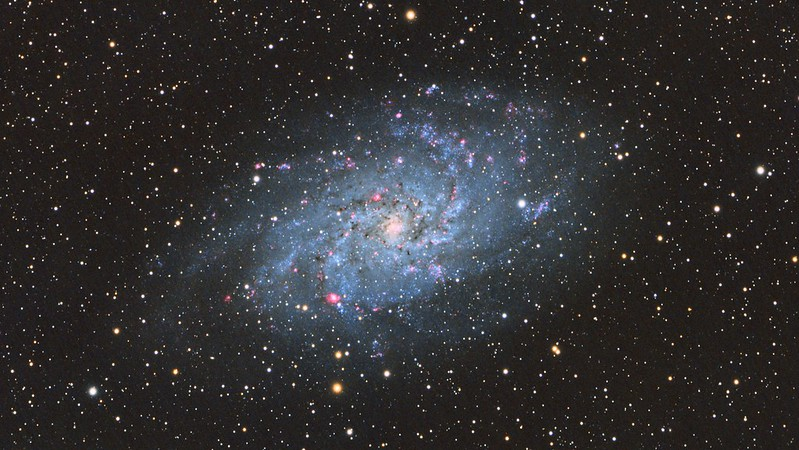
\includegraphics[width=0.8\textwidth]{capitulo-1/28421613139_a4472645e5_c.jpg}
    \caption[Galáxia M33]{Galáxia do Triângulo M33.}
\end{figure}

\subsection{Múltiplas figuras}

\begin{figure}[t]
    \centering
    \begin{subfigure}[b]{0.3\textwidth}
        \centering
        \includegraphics[width=\textwidth]{example-image-duck}
        \caption{Primeiro pato.}
    \end{subfigure}
    \hfill
    \begin{subfigure}[b]{0.3\textwidth}
        \centering
        \includegraphics[width=\textwidth]{example-image-duck}
        \caption{Segundo pato.}
    \end{subfigure}
    \hfill
    \begin{subfigure}[b]{0.3\textwidth}
        \centering
        \includegraphics[width=\textwidth]{example-image-duck}
        \caption{Terceiro pato.}
    \end{subfigure}
       \caption{Três patos juntos.}
\end{figure}
